\documentclass[addpoints,spanish, 12pt,a4paper]{exam}
%\documentclass[answers, spanish, 12pt,a4paper]{exam}
% \printanswers
\pointpoints{punto}{puntos}
\hpword{Puntos:}
\vpword{Puntos:}
\htword{Total}
\vtword{Total}
\hsword{Resultado:}
\hqword{Ejercicio:}
\vqword{Ejercicio:}

\usepackage[utf8]{inputenc}
\usepackage[spanish]{babel}
\usepackage{eurosym}
%\usepackage[spanish,es-lcroman, es-tabla, es-noshorthands]{babel}


\usepackage[margin=1in]{geometry}
\usepackage{amsmath,amssymb}
\usepackage{multicol}
\usepackage{yhmath}

\pointsinrightmargin % Para poner las puntuaciones a la derecha. Se puede cambiar. Si se comenta, sale a la izquierda.
\extrawidth{-2.4cm} %Un poquito más de margen por si ponemos textos largos.
\marginpointname{ \emph{\points}}

\usepackage{graphicx}

\graphicspath{{../../img/}} 

\newcommand{\class}{2º Bachillerato CIT}
\newcommand{\examdate}{\today}
\newcommand{\examnum}{Parcial 1ªEv.}
\newcommand{\tipo}{B}


\newcommand{\timelimit}{45 minutos}

\renewcommand{\solutiontitle}{\noindent\textbf{Solución:}\enspace}


\pagestyle{head}
\firstpageheader{
\includegraphics[width=0.2\columnwidth]{header_left}}{\textbf{Departamento de Matemáticas\linebreak \class}\linebreak \examnum}{
\includegraphics[width=0.1\columnwidth]{header_right}}
\runningheader{\class}{\examnum}{Página \thepage\ of \numpages}
\runningheadrule


\usepackage{pgf,tikz,pgfplots}
\pgfplotsset{compat=1.15}
\usepackage{mathrsfs}
\usetikzlibrary{arrows}


\begin{document}

\noindent
\begin{tabular*}{\textwidth}{l @{\extracolsep{\fill}} r @{\extracolsep{6pt}} }
\textbf{Nombre:} \makebox[3.5in]{\hrulefill} & \textbf{Fecha:}\makebox[1in]{\hrulefill} \\
 & \\
\textbf{Tiempo: \timelimit} & Tipo: \tipo 
\end{tabular*}
\rule[2ex]{\textwidth}{2pt}
Esta prueba tiene \numquestions\ ejercicios. La puntuación máxima es de \numpoints. 
La nota final de la prueba será la parte proporcional de la puntuación obtenida sobre la puntuación máxima. 

\begin{center}


\addpoints
 %\gradetable[h][questions]
	\pointtable[h][questions]
\end{center}

\noindent
\rule[2ex]{\textwidth}{2pt}

\begin{questions}

%\question 
%
%\begin{parts}
%\part[2] 
%\begin{solution}
%\end{solution}
%
%
%\end{parts}
%\addpoints

% \question[1] Calcula el siguiente límite:

% $$\lim_{x \to 1}\left(\frac{1 - \sqrt{2 - x}}{x^{2} - 3 x + 2}\right)$$

% \begin{solution}$- \frac{1}{2}$\end{solution}

\question[1] Calcula el siguiente límite:

$$\lim_{x \to 3}\left(\frac{2 - \sqrt{1 + x}}{x -3}\right)$$

\begin{solution}$- \frac{1}{4}$\end{solution}

% \question[1] Calcula el siguiente límite:

% $$\lim_{x \to \infty} \left(\frac{x + 5}{x - 1}\right)^{2 x + 1}$$

% \begin{solution}$e^{12}$\end{solution}

\question[1] Calcula el siguiente límite:

$$\lim_{x \to \infty} \left(\frac{x + 2}{x - 3}\right)^{2 x}$$

\begin{solution}$e^{10}$\end{solution}

\question Sea la función: $$g(x)=\dfrac{x^2-4}{x-2}$$
\begin{parts}
\part[1] Estudia la continuidad de la función
\begin{solution}$\mathbb{R}-\left\{ 2\right\}=\left(-\infty,2\right)\cup \left(2,\infty\right)
$\end{solution}

\part[2] Redefine la función para que sea continua en $\mathbb{R}$
\begin{solution} $f(x)=\left\{ \begin{array}{ccl} \dfrac{x^2-4}{x-2} & , & x \neq 2 \\ 4 & , & x=2 \end{array} \right.$ \end{solution}
\end{parts}

% \question Dada la función:
% $$f(x)=\left\{ \begin{array}{ccl} \dfrac{e^{-x}}{2} & , & x < 0 \\ & \\ -x^2+k & , & x\geqslant 0 \end{array} \right.$$
% \begin{parts}
% \part[1] Calcula el valor de $k$ para que la función sea continua
% \begin{solution}
% $k=\frac{1}{2}$
% \end{solution}
% \part[2] Representa gráficamente la función.
% \begin{solution}
% 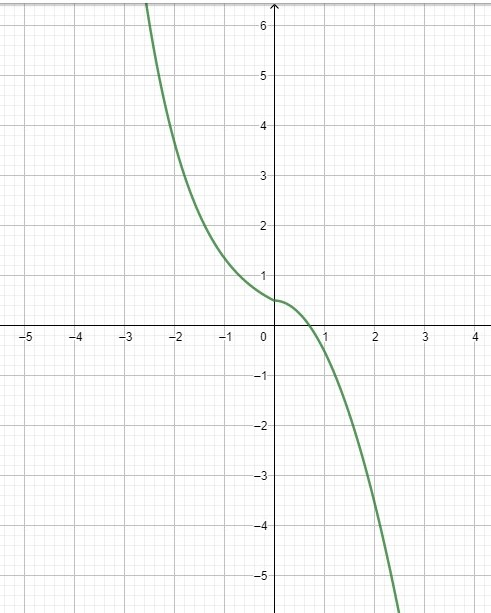
\includegraphics[width=0.3\columnwidth]{funcion1}
% \end{solution}
% \end{parts}

\question Dada la función:
$$f(x)=\dfrac{x^2+5x+3}{x+2}$$
\begin{parts}
\part[2] Calcula las asíntotas
\begin{solution}
$x=-2$ y $y=x+3$
\end{solution}
\part[1] Determina si la gráfica corta a alguna de las asíntotas
\begin{solution}
No corta a ninguna
\end{solution}
\end{parts}		

% \question Dada la función:
% $$f(x)=\dfrac{x^3-2x+1}{x^2-1}$$
% \begin{parts}
% \part[2] Calcula las asíntotas
% \begin{solution}
% $f(x)=\frac{\left(x - 1\right) \left(x^{2} + x - 1\right)}{(x+1)(x-1)}$ \\
% $x=-1$ y $y=x$
% \end{solution}
% \part[1] Determina si la gráfica corta a alguna de las asíntotas
% \begin{solution}
% No corta a ninguna
% \end{solution}
% \end{parts}		




\addpoints

\end{questions}

\end{document}
\grid
